% Options for packages loaded elsewhere
% Options for packages loaded elsewhere
\PassOptionsToPackage{unicode}{hyperref}
\PassOptionsToPackage{hyphens}{url}
\PassOptionsToPackage{dvipsnames,svgnames,x11names}{xcolor}
%
\documentclass[
  letterpaper,
  DIV=11,
  numbers=noendperiod]{scrreprt}
\usepackage{xcolor}
\usepackage{amsmath,amssymb}
\setcounter{secnumdepth}{5}
\usepackage{iftex}
\ifPDFTeX
  \usepackage[T1]{fontenc}
  \usepackage[utf8]{inputenc}
  \usepackage{textcomp} % provide euro and other symbols
\else % if luatex or xetex
  \usepackage{unicode-math} % this also loads fontspec
  \defaultfontfeatures{Scale=MatchLowercase}
  \defaultfontfeatures[\rmfamily]{Ligatures=TeX,Scale=1}
\fi
\usepackage{lmodern}
\ifPDFTeX\else
  % xetex/luatex font selection
\fi
% Use upquote if available, for straight quotes in verbatim environments
\IfFileExists{upquote.sty}{\usepackage{upquote}}{}
\IfFileExists{microtype.sty}{% use microtype if available
  \usepackage[]{microtype}
  \UseMicrotypeSet[protrusion]{basicmath} % disable protrusion for tt fonts
}{}
\makeatletter
\@ifundefined{KOMAClassName}{% if non-KOMA class
  \IfFileExists{parskip.sty}{%
    \usepackage{parskip}
  }{% else
    \setlength{\parindent}{0pt}
    \setlength{\parskip}{6pt plus 2pt minus 1pt}}
}{% if KOMA class
  \KOMAoptions{parskip=half}}
\makeatother
% Make \paragraph and \subparagraph free-standing
\makeatletter
\ifx\paragraph\undefined\else
  \let\oldparagraph\paragraph
  \renewcommand{\paragraph}{
    \@ifstar
      \xxxParagraphStar
      \xxxParagraphNoStar
  }
  \newcommand{\xxxParagraphStar}[1]{\oldparagraph*{#1}\mbox{}}
  \newcommand{\xxxParagraphNoStar}[1]{\oldparagraph{#1}\mbox{}}
\fi
\ifx\subparagraph\undefined\else
  \let\oldsubparagraph\subparagraph
  \renewcommand{\subparagraph}{
    \@ifstar
      \xxxSubParagraphStar
      \xxxSubParagraphNoStar
  }
  \newcommand{\xxxSubParagraphStar}[1]{\oldsubparagraph*{#1}\mbox{}}
  \newcommand{\xxxSubParagraphNoStar}[1]{\oldsubparagraph{#1}\mbox{}}
\fi
\makeatother


\usepackage{longtable,booktabs,array}
\usepackage{calc} % for calculating minipage widths
% Correct order of tables after \paragraph or \subparagraph
\usepackage{etoolbox}
\makeatletter
\patchcmd\longtable{\par}{\if@noskipsec\mbox{}\fi\par}{}{}
\makeatother
% Allow footnotes in longtable head/foot
\IfFileExists{footnotehyper.sty}{\usepackage{footnotehyper}}{\usepackage{footnote}}
\makesavenoteenv{longtable}
\usepackage{graphicx}
\makeatletter
\newsavebox\pandoc@box
\newcommand*\pandocbounded[1]{% scales image to fit in text height/width
  \sbox\pandoc@box{#1}%
  \Gscale@div\@tempa{\textheight}{\dimexpr\ht\pandoc@box+\dp\pandoc@box\relax}%
  \Gscale@div\@tempb{\linewidth}{\wd\pandoc@box}%
  \ifdim\@tempb\p@<\@tempa\p@\let\@tempa\@tempb\fi% select the smaller of both
  \ifdim\@tempa\p@<\p@\scalebox{\@tempa}{\usebox\pandoc@box}%
  \else\usebox{\pandoc@box}%
  \fi%
}
% Set default figure placement to htbp
\def\fps@figure{htbp}
\makeatother


% definitions for citeproc citations
\NewDocumentCommand\citeproctext{}{}
\NewDocumentCommand\citeproc{mm}{%
  \begingroup\def\citeproctext{#2}\cite{#1}\endgroup}
\makeatletter
 % allow citations to break across lines
 \let\@cite@ofmt\@firstofone
 % avoid brackets around text for \cite:
 \def\@biblabel#1{}
 \def\@cite#1#2{{#1\if@tempswa , #2\fi}}
\makeatother
\newlength{\cslhangindent}
\setlength{\cslhangindent}{1.5em}
\newlength{\csllabelwidth}
\setlength{\csllabelwidth}{3em}
\newenvironment{CSLReferences}[2] % #1 hanging-indent, #2 entry-spacing
 {\begin{list}{}{%
  \setlength{\itemindent}{0pt}
  \setlength{\leftmargin}{0pt}
  \setlength{\parsep}{0pt}
  % turn on hanging indent if param 1 is 1
  \ifodd #1
   \setlength{\leftmargin}{\cslhangindent}
   \setlength{\itemindent}{-1\cslhangindent}
  \fi
  % set entry spacing
  \setlength{\itemsep}{#2\baselineskip}}}
 {\end{list}}
\usepackage{calc}
\newcommand{\CSLBlock}[1]{\hfill\break\parbox[t]{\linewidth}{\strut\ignorespaces#1\strut}}
\newcommand{\CSLLeftMargin}[1]{\parbox[t]{\csllabelwidth}{\strut#1\strut}}
\newcommand{\CSLRightInline}[1]{\parbox[t]{\linewidth - \csllabelwidth}{\strut#1\strut}}
\newcommand{\CSLIndent}[1]{\hspace{\cslhangindent}#1}



\setlength{\emergencystretch}{3em} % prevent overfull lines

\providecommand{\tightlist}{%
  \setlength{\itemsep}{0pt}\setlength{\parskip}{0pt}}



 


\KOMAoption{captions}{tableheading}
\makeatletter
\@ifpackageloaded{bookmark}{}{\usepackage{bookmark}}
\makeatother
\makeatletter
\@ifpackageloaded{caption}{}{\usepackage{caption}}
\AtBeginDocument{%
\ifdefined\contentsname
  \renewcommand*\contentsname{Table of contents}
\else
  \newcommand\contentsname{Table of contents}
\fi
\ifdefined\listfigurename
  \renewcommand*\listfigurename{List of Figures}
\else
  \newcommand\listfigurename{List of Figures}
\fi
\ifdefined\listtablename
  \renewcommand*\listtablename{List of Tables}
\else
  \newcommand\listtablename{List of Tables}
\fi
\ifdefined\figurename
  \renewcommand*\figurename{Figure}
\else
  \newcommand\figurename{Figure}
\fi
\ifdefined\tablename
  \renewcommand*\tablename{Table}
\else
  \newcommand\tablename{Table}
\fi
}
\@ifpackageloaded{float}{}{\usepackage{float}}
\floatstyle{ruled}
\@ifundefined{c@chapter}{\newfloat{codelisting}{h}{lop}}{\newfloat{codelisting}{h}{lop}[chapter]}
\floatname{codelisting}{Listing}
\newcommand*\listoflistings{\listof{codelisting}{List of Listings}}
\makeatother
\makeatletter
\makeatother
\makeatletter
\@ifpackageloaded{caption}{}{\usepackage{caption}}
\@ifpackageloaded{subcaption}{}{\usepackage{subcaption}}
\makeatother
\usepackage{bookmark}
\IfFileExists{xurl.sty}{\usepackage{xurl}}{} % add URL line breaks if available
\urlstyle{same}
\hypersetup{
  pdftitle={Regulation of MAPT (Tau) Translation in Basal Forebrain Axons},
  pdfauthor={Elina Nemtsov},
  colorlinks=true,
  linkcolor={blue},
  filecolor={Maroon},
  citecolor={Blue},
  urlcolor={Blue},
  pdfcreator={LaTeX via pandoc}}


\title{Regulation of MAPT (Tau) Translation in Basal Forebrain Axons}
\author{Elina Nemtsov}
\date{2026-03-09}
\begin{document}
\maketitle

\renewcommand*\contentsname{Table of contents}
{
\hypersetup{linkcolor=}
\setcounter{tocdepth}{2}
\tableofcontents
}

\bookmarksetup{startatroot}

\chapter{}\label{section}

\bookmarksetup{startatroot}

\chapter*{Abstract}\label{abstract}
\addcontentsline{toc}{chapter}{Abstract}

\markboth{Abstract}{Abstract}

Short summary - do last

\bookmarksetup{startatroot}

\chapter*{Acknowledgements}\label{acknowledgements}
\addcontentsline{toc}{chapter}{Acknowledgements}

\markboth{Acknowledgements}{Acknowledgements}

Your acknowledgements here.

\bookmarksetup{startatroot}

\chapter*{List of Abbreviations}\label{list-of-abbreviations}
\addcontentsline{toc}{chapter}{List of Abbreviations}

\markboth{List of Abbreviations}{List of Abbreviations}

\begin{itemize}
\tightlist
\item
  LC --- Locus Coeruleus
\item
  p75NTR --- p75 Neurotrophin Receptor
\end{itemize}

\bookmarksetup{startatroot}

\chapter{Background}\label{background}

Traumatic brain injury (TBI) is traditionally viewed as a focal insult,
in which neurons at the site of impact undergo acute necrotic or
apoptotic cell death. However, it is now well established that the
consequences of brain injury extend far beyond the cortical neurons
directly affected by the initial trauma. Injury to the cortex induces
profound and long-lasting changes in the local extracellular
environment, including inflammation, altered neurotrophin availability,
and disruption of synaptic homeostasis. These changes can propagate
retrogradely to afferent neuronal populations that project to the
injured region, leading to delayed and secondary degeneration that
unfolds over days to weeks after the initial injury.

Basal forebrain cholinergic neurons (BFCNs), which send extensive axonal
projections to the cerebral cortex, undergo retrograde degeneration
following cortical TBI despite the absence of direct mechanical damage
to their cell bodies (\citeproc{ref-Counts2011}{Counts and Mufson 2011};
\citeproc{ref-dasguptaProNGFElicitsRetrograde2024}{Dasgupta et al.
2024}). Importantly, this degeneration is mediated by signaling events
initiated at the distal axon terminals within the injured cortex, rather
than by intrinsic somatic damage
(\citeproc{ref-dasguptaProNGFElicitsRetrograde2024}{Dasgupta et al.
2024}). The signal that mediates this is an increase in the amount of
the immature proform of nerve growth factor (proNGF) in the cerebral
cortex, this results in retrograde degeneration of BFCNs through
activation of proNGF receptor p75NTR. In addition, previous work from
the lab showed that that local axonal protein synthesis and retrograde
transport mediated proNGF-induced degeneration which was initiated at
the axon terminal
(\citeproc{ref-dasguptaProNGFElicitsRetrograde2024}{Dasgupta et al.
2024}).

This thesis builds on this framework by focusing on the molecular
mechanisms that link cortical injury to retrograde axonal degeneration
in BFCNs. In particular, it examines the role of the p75 neurotrophin
receptor (p75NTR), a receptor that is persistently expressed in adult
BFCNs (\citeproc{ref-Yaar1997}{Yaar et al. 1997}) and is strongly
implicated in injury-induced and stress-induced degeneration
(\citeproc{ref-Ibanez1992}{Ibáñez 1992}). While p75NTR signaling has
been extensively studied in the context of neurodegenerative disease,
increasing evidence indicates that it plays a critical role in secondary
degeneration after TBI. Moreover, TBI is now recognized as a major risk
factor for the later development of neurodegenerative diseases,
suggesting that shared molecular pathways may underlie both
injury-induced and disease-associated neuronal loss.

Within this context, Tau (microtubule-associated protein Tau, MAPT)
emerges as a compelling candidate mediator of p75NTR-dependent axonal
degeneration. Tau has classically been studied in neurodegenerative
disease, particularly Alzheimer's disease (\citeproc{ref-Lei2016}{Lei et
al. 2016}), but its functions in axonal signaling, transport, and injury
responses are increasingly appreciated. This introduction therefore
emphasizes traumatic brain injury as the initiating event, with
neurodegenerative disease discussed as a related and downstream
consequence, and frames Tau as a potential signaling effector linking
p75NTR activation to axonal fragmentation in BFCNs.

\section{Traumatic Brain Injury and Secondary Retrograde
Neurodegeneration}\label{traumatic-brain-injury-and-secondary-retrograde-neurodegeneration}

Traumatic brain injury results in immediate damage at the site of
impact, characterized by mechanical disruption of neurons, glia, and
vasculature. In addition to this primary injury, a secondary phase
ensues in which biochemical and molecular changes propagate through
connected neural circuits. These secondary processes include
neuroinflammation, excitotoxicity, oxidative stress, and alterations in
trophic support. Importantly, neurons that project to the injured cortex
experience a sudden loss or imbalance of target-derived signals,
exposing their distal axons to a hostile environment despite the
physical separation of their somata from the injury site.

Experimental models of cortical injury have demonstrated that afferent
neuronal populations undergo delayed degeneration as a result of these
secondary changes. This retrograde degeneration is not a passive
consequence of axotomy but rather a regulated process involving
receptor-mediated signaling at the axon terminal, retrograde transport
of injury signals, and activation of stress-responsive pathways
(\citeproc{ref-dasguptaProNGFElicitsRetrograde2024}{Dasgupta et al.
2024}). Such mechanisms are particularly relevant for neuromodulatory
neurons with long, highly branched axons, including BFCNs.

\section{Neurotrophin Signaling and p75NTR in Injury-Induced
Degeneration}\label{neurotrophin-signaling-and-p75ntr-in-injury-induced-degeneration}

Neurotrophins are key regulators of neuronal survival and maintenance,
and their signaling balance is profoundly disrupted after brain injury
(\citeproc{ref-Dechant2002}{Dechant and Barde 2002};
\citeproc{ref-Kaplan2013}{Kaplan and Miller, n.d.}). All neurotrophins
are synthesized as precursor proneurotrophins, which can be cleaved to
generate mature ligands with distinct biological functions. After TBI,
there is a well-documented shift in the injured cortex toward increased
levels of proneurotrophins, including proNGF and proBDNF, relative to
their mature counterparts (\citeproc{ref-Counts2011}{Counts and Mufson
2011}).

Proneurotrophins bind with high affinity to p75NTR, particularly in
complexes containing sortilin, and preferentially activate degenerative
signaling pathways (\citeproc{ref-Teng2005}{Helen K. Teng et al. 2005};
\citeproc{ref-tengProBDNFInducesNeuronal2005}{Henry K. Teng et al.
2005}). Activation of p75NTR initiates intracellular cascades involving
adaptor proteins and stress kinases, most notably c-Jun N-terminal
kinase (JNK) (\citeproc{ref-Ibanez1992}{Ibáñez 1992};
\citeproc{ref-Dechant2002}{Dechant and Barde 2002}). p75NTR--JNK
signaling has been implicated in both apoptotic cell death and axonal
degeneration, and critically, this signaling can be initiated locally at
axon terminals and transmitted retrogradely to the soma
(\citeproc{ref-dasguptaProNGFElicitsRetrograde2024}{Dasgupta et al.
2024}).

p75NTR has been shown to contribute to secondary degeneration in the
penumbra following cortical TBI, and genetic or pharmacological
disruption of p75NTR signaling confers protection to projecting neurons
(\citeproc{ref-dasguptaProNGFElicitsRetrograde2024}{Dasgupta et al.
2024}). These findings position p75NTR as a central mediator linking
cortical injury to retrograde neuronal degeneration.

\section{Basal Forebrain Cholinergic Neurons as a Model of Retrograde
Vulnerability}\label{basal-forebrain-cholinergic-neurons-as-a-model-of-retrograde-vulnerability}

Basal forebrain cholinergic neurons provide widespread cholinergic
innervation to the cortex and hippocampus and are essential for
cognitive functions such as attention, learning, and memory. A defining
feature of BFCNs is their continued expression of p75NTR throughout
adulthood, distinguishing them from many other central neurons
(\citeproc{ref-Yaar1997}{Yaar et al. 1997}).

Following cortical injury, BFCNs exhibit axonal degeneration and loss
that is ipsilateral to the site of injury, despite the absence of direct
trauma to the basal forebrain (\citeproc{ref-Counts2011}{Counts and
Mufson 2011};
\citeproc{ref-dasguptaProNGFElicitsRetrograde2024}{Dasgupta et al.
2024}). In vitro compartmentalized culture systems have demonstrated
that activation of p75NTR specifically at BFCN axon terminals is
sufficient to induce axonal fragmentation and retrograde cell death
(\citeproc{ref-dasguptaProNGFElicitsRetrograde2024}{Dasgupta et al.
2024}). Notably, axonal degeneration often precedes somatic apoptosis,
indicating that axons are an early and primary target of injury-induced
signaling.

These properties make BFCNs an ideal model system for dissecting the
molecular mechanisms of retrograde degeneration initiated by cortical
injury.

\section{Tau background and roles}\label{tau-background-and-roles}

Tau is a microtubule-associated protein that stabilizes axonal
microtubules and regulates cytoskeletal dynamics under physiological
conditions. Beyond its structural role, tau participates in axonal
transport regulation and can act as a phosphorylation-state-dependent
scaffold that links signaling to trafficking and synaptic function.
(Review: https://www.mdpi.com/1422-0067/22/17/9207)

\subsection{Core roles of Tau}\label{core-roles-of-tau}

\begin{itemize}
\tightlist
\item
  \textbf{Microtubule stabilization and cytoskeletal coordination}

  \begin{itemize}
  \tightlist
  \item
    Binds and stabilizes axonal microtubules to maintain neuronal
    polarity and cytoskeletal integrity. (Review:
    https://www.mdpi.com/1422-0067/22/17/9207)
  \item
    Coordinates microtubule--actin network behavior to support axonal
    structure and dynamics. (Review:
    https://www.mdpi.com/1422-0067/22/17/9207)
  \end{itemize}
\item
  \textbf{Regulation of axonal transport}

  \begin{itemize}
  \tightlist
  \item
    Supports efficient bidirectional trafficking by tuning the
    accessibility of microtubule tracks for kinesin/dynein-driven cargo
    movement. (Review: https://www.mdpi.com/1422-0067/22/17/9207)
  \item
    Under pathological conditions, hyperphosphorylated tau can
    trap/perturb motor-adaptor complexes (e.g., JIP1--kinesin),
    disrupting cargo-selective transport. (Primary:
    https://pmc.ncbi.nlm.nih.gov/articles/PMC2742856/ ; PMID landing
    page: https://pubmed.ncbi.nlm.nih.gov/19491104/)
  \end{itemize}
\item
  \textbf{Signaling scaffold (stress and kinase signaling integration)}

  \begin{itemize}
  \tightlist
  \item
    Organizes kinase/stress-response pathways and can link extracellular
    cues to intracellular responses in a phospho-state-dependent manner.
    (Review: https://www.mdpi.com/1422-0067/22/17/9207)
  \end{itemize}
\item
  \textbf{Synaptic function and plasticity}

  \begin{itemize}
  \tightlist
  \item
    Modulates synaptic vesicle cycling and postsynaptic processes,
    consistent with tau's presence in dendritic spines and synaptic
    compartments. (Review: https://www.mdpi.com/1422-0067/22/17/9207)
  \item
    Contributes to dynamic \textbf{AMPAR trafficking} in dendrites,
    influencing synaptic efficacy. (Primary example:
    https://pubmed.ncbi.nlm.nih.gov/28554859/)
  \end{itemize}
\item
  \textbf{Proteostasis and clearance}

  \begin{itemize}
  \tightlist
  \item
    Interfaces with chaperones, proteasome, and autophagy machinery to
    regulate tau turnover and quality control. (Review:
    https://www.mdpi.com/1422-0067/22/17/9207)
  \end{itemize}
\item
  \textbf{Nuclear and stress-related roles}

  \begin{itemize}
  \tightlist
  \item
    A smaller nuclear fraction can bind DNA and may contribute to
    protection against stress-induced DNA damage. (Review:
    https://www.mdpi.com/1422-0067/22/17/9207)
  \end{itemize}
\end{itemize}

\subsection{Tau interaction with the dynein--dynactin transport
machinery}\label{tau-interaction-with-the-dyneindynactin-transport-machinery}

Of particular interest to our research is tau's ability to regulate
axonal transport by interacting with components of the dynein--dynactin
motor complex. A previous study demonstrated that the N-terminal
projection domain of tau binds the C-terminal region of the p150 subunit
of dynactin, a key activator of the dynein motor responsible for
retrograde transport along microtubules
(\citeproc{ref-magnaniInteractionTauProtein2007}{\textbf{magnaniInteractionTauProtein2007?}}).
Through this interaction, tau can simultaneously bind microtubules via
its C-terminal repeat domain while recruiting the dynactin complex
through its N-terminal projection domain. This structural arrangement
positions tau as a molecular scaffold that stabilizes the association of
the dynein--dynactin transport machinery with axonal microtubules,
thereby supporting efficient cargo transport.

Consistent with this model, the authors showed that the presence of tau
increases the association of the dynactin complex with microtubules in
vitro, suggesting that tau helps stabilize transport complexes on the
microtubule lattice. Importantly, this interaction occurs through
sequences encoded by exons 1--4 of the tau protein, indicating that the
N-terminal projection domain mediates the dynactin interaction while the
microtubule-binding repeats anchor tau to the microtubule cytoskeleton.
The neuronal model used in this study expressed only the 0N3R and 0N4R
tau isoforms which lack exons 2 and 3. As reported by the authors:
\emph{``SH-SY5Y cells express only the shortest three- and four-repeat
tau isoforms without amino-terminal inserts.''} Despite this, dynactin
p150 was still found to co-immunoprecipitate with tau, showing that the
absence of N-terminal inserts does not impair the ability of tau to bind
dynactin. This observation is particularly relevant to our experimental
neuronal culture systems that showed similar tau isoforms present. This
dual role of tau in microtubule stabilization and transport regulation
is particularly relevant in the context of axonal injury and
degeneration, where disruptions in either function can either prevent or
contribute to axon degeneration and cell death. Our labs previous study
showed that blocking dynein-dependent retrograde transport with the
inhibitor ``ciliobrevin D'' prevented both axon degeneration and
neuronal death induced by axonal proNGF stimulation
(\citeproc{ref-dasguptaProNGFElicitsRetrograde2024}{Dasgupta et al.
2024}). These results indicate that degenerative signals initiated at
the axon terminal must be transported retrogradely to the soma to
execute the degeneration program. Together with study showing that tau
interacts with the dynactin--dynein motor complex, it is possible that
tau contributes to the regulation of retrograde signaling by
facilitating the association of the dynein--dynactin transport machinery
with microtubules. Thus, the local translation upregulation of tau
functions to stabilize the efficiency of retrograde transport to allow
axonal degeneration.

\subsection{When Tau becomes
pathological}\label{when-tau-becomes-pathological}

When tau becomes excessively phosphorylated, it detaches from
microtubules, destabilizes cytoskeletal organization and axonal
transport, and becomes prone to misfolding and aggregation into
oligomers/paired helical filaments and neurofibrillary tangles, a
pathological hallmark of Alzheimer's disease and other tauopathies.
(Review: https://www.mdpi.com/1422-0067/22/17/9207)

\subsection{Post-translational modifications and why phosphorylation
matters}\label{post-translational-modifications-and-why-phosphorylation-matters}

Tau's functional ``mode'' is strongly shaped by post-translational
modifications (PTMs), including phosphorylation, acetylation,
truncation, ubiquitination, glycation, and others. These PTMs can change
tau's microtubule affinity, subcellular localization, interactions with
motors/adaptors, and aggregation propensity. (Review:
https://www.mdpi.com/1422-0067/22/17/9207)

Phosphorylation is especially important because it can directly weaken
tau--microtubule binding and shift tau toward conformations and
interaction networks that impair trafficking and favor aggregation.
Site-specific phosphorylation patterns are also leveraged as biomarkers
(CSF/plasma) and neuropathology readouts. (Review overview of
phosphorylation patterns/biomarkers:
https://pmc.ncbi.nlm.nih.gov/articles/PMC10839341/)

\subsection{Antibodies used in this study (tau phosphorylation
readouts)}\label{antibodies-used-in-this-study-tau-phosphorylation-readouts}

In this research, I quantified tau phosphorylation using three
antibodies that report distinct tau states:

\begin{itemize}
\item
  \textbf{pThr181 (p-tau181)}: commonly used biomarker-associated
  phosphorylation site that tracks Alzheimer's disease-related tau
  pathology in CSF and plasma and is widely used for
  staging/stratification. (Context review:
  https://pmc.ncbi.nlm.nih.gov/articles/PMC10839341/)
\item
  \textbf{AT8 (pSer202/pThr205)}: canonical neuropathology epitope used
  to detect early and established pathological tau (pre-tangles/tangles)
  in tissue; often treated as a marker of disease-associated tau
  phosphorylation. (Epitope/usage context:
  https://www.alzforum.org/alzantibodies/tau-at8-phospho-tau-ser-202-thr-205)
\item
  \textbf{pSer622}: a C-terminal tau site sometimes assessed in
  biochemical studies; interpretation can depend on antibody specificity
  and isoform context, and is typically considered alongside broader
  phosphorylation patterns rather than as a standalone ``core
  biomarker'' site. (Phosphorylation landscape context:
  https://pmc.ncbi.nlm.nih.gov/articles/PMC10839341/)
\end{itemize}

\section{proNGF--p75NTR signaling and tau
phosphorylation}\label{prongfp75ntr-signaling-and-tau-phosphorylation}

A central focus of this thesis is how \textbf{proNGF--p75NTR signaling}
engages stress-associated kinase cascades that converge on tau
phosphorylation states linked to axonal dysfunction and degeneration.

Genetic deletion of p75NTR attenuates tau hyperphosphorylation in a
tauopathy mouse model, and p75NTR is required for ligand-driven tau
phosphorylation in vitro, supporting a causal role for p75NTR signaling
in tau phosphorylation pathways. (Primary:
https://pmc.ncbi.nlm.nih.gov/articles/PMC6756909/ ; PubMed:
https://pubmed.ncbi.nlm.nih.gov/31479419/)

Mechanistically, p75NTR activation can engage downstream kinases
including \textbf{JNK}, a stress-activated MAPK family member with
well-described roles in neurodegenerative signaling. JNK isoforms can
phosphorylate tau at multiple sites and influence tau's interaction
landscape, consistent with a model where p75NTR-dependent stress
signaling drives tau modifications that destabilize the axonal
cytoskeleton and transport. (JNK--tau biochemical/kinase context:
https://pubs.acs.org/doi/10.1021/acschemneuro.3c00093)

Tau is also positioned to integrate signaling and transport because
under pathological conditions hyperphosphorylated tau interacts with the
JNK scaffold/adaptor \textbf{JIP1}, which associates with kinesin motor
complexes; this interaction disrupts kinesin motor complex formation and
is linked to axonal transport defects. (Primary:
https://pmc.ncbi.nlm.nih.gov/articles/PMC2742856/ ; PubMed:
https://pubmed.ncbi.nlm.nih.gov/19491104/)

Importantly, several kinases activated downstream of p75NTR signaling,
including JNK, directly phosphorylate Tau at sites associated with
axonal degeneration (\citeproc{ref-Lei2016}{Lei et al. 2016}). Tau also
interacts with motor proteins and components of the retrograde transport
machinery, positioning it as a potential scaffold that integrates
signaling and transport processes within the axon
(\citeproc{ref-Morfini2009}{Morfini et al. 2009}).

\subsection{Linking p75NTR Signaling, Tau, and Axonal Fragmentation
After
TBI}\label{linking-p75ntr-signaling-tau-and-axonal-fragmentation-after-tbi}

Recent work from our laboratory has demonstrated that proneurotrophin
stimulation of BFCN axons induces local axonal protein synthesis,
retrograde transport of degenerative signals, and axonal fragmentation
through p75NTR-dependent mechanisms
(\citeproc{ref-dasguptaProNGFElicitsRetrograde2024}{Dasgupta et al.
2024}; \citeproc{ref-cagnettaRapidCueSpecificRemodeling2018}{Cagnetta et
al. 2018}). These findings identify axons as active sites of signal
integration rather than passive conduits.

Within this framework, Tau is well positioned to act as a downstream
effector of p75NTR signaling. By modulating microtubule stability,
axonal transport, and cytoskeletal organization, Tau may translate
p75NTR--JNK signaling into the structural breakdown of axons observed
after cortical injury. This raises the possibility that Tau is not
merely a marker of degeneration but an active participant in
injury-induced axonal fragmentation.

\section{Scope and Aims of Thesis}\label{scope-and-aims-of-thesis}

The overarching goal of this thesis is to define the role of Tau in
p75NTR-mediated degeneration and axonal fragmentation of basal forebrain
cholinergic neurons following cortical injury. Specifically, this work
aims to:

\begin{enumerate}
\def\labelenumi{\arabic{enumi}.}
\tightlist
\item
  Characterize p75NTR-dependent signaling in BFCNs after axonal proNGF
  treatment specifically is ``Tau synthesis increase upstream or
  downstream of APP?'' Is newely synthesized Tau required for
  p75NTR-induced axonal degeneration and fragmentation?
\item
  Does blocking new APP synthesis will prevent Tau increase and axonal
  degeneration?
\item
  Characterize levels of total Tau and phosphorylated Tau after proNGF
  treatment, is proNGF treatment increases a specific phospho-Tau
  species that is associated with axonal degeneration?
\end{enumerate}

\bookmarksetup{startatroot}

\chapter{Results}\label{results}

\section{September 2025 --- proNGF Time
Course}\label{september-2025-prongf-time-course}

\textbf{Conditions:} Ctrl · ProNGF 30 min · ProNGF 45 min · ProNGF 60
min \textbf{Antibodies:} Tau (DyLight 800, 56 kDa) · Actin (DyLight 800,
42 kDa)

\subsection{Blot Images}\label{blot-images}

\begin{figure}[H]

{\centering 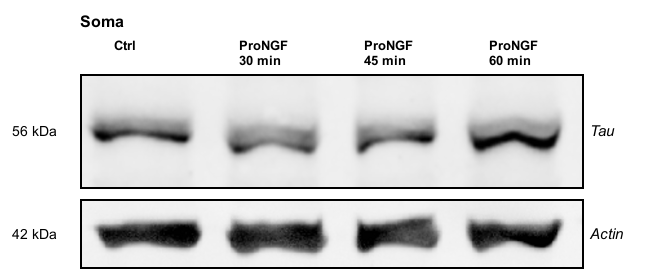
\includegraphics[width=0.8\linewidth,height=\textheight,keepaspectratio]{figures/sep-show-soma-1.png}

}

\caption{September 2025 --- Soma compartment. Tau (56 kDa) and Actin (42
kDa), DyLight 800.}

\end{figure}%

\begin{figure}[H]

{\centering 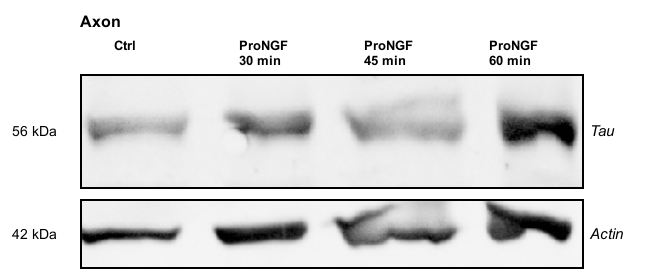
\includegraphics[width=0.8\linewidth,height=\textheight,keepaspectratio]{figures/sep-show-axon-1.png}

}

\caption{September 2025 --- Axon compartment. Tau (56 kDa) and Actin (42
kDa), DyLight 800.}

\end{figure}%

\subsection{Quantification}\label{quantification}

\begin{figure}[H]

{\centering \includegraphics[width=0.8\linewidth,height=\textheight,keepaspectratio]{figures/sep-ratio-1.pdf}

}

\caption{September 2025 --- Tau / Actin ratio in soma and axon
compartments across proNGF treatment conditions.}

\end{figure}%

\begin{figure}[H]

{\centering \includegraphics[width=0.8\linewidth,height=\textheight,keepaspectratio]{figures/sep-raw-1.pdf}

}

\caption{September 2025 --- Raw Tau and Actin band intensities.}

\end{figure}%

\begin{center}\rule{0.5\linewidth}{0.5pt}\end{center}

\section{February 2026 --- 1st Western Blot (Axon \&
Soma)}\label{february-2026-1st-western-blot-axon-soma}

\textbf{Conditions:} Ctrl (soma only) · ProNGF 45 min · ProNGF 60 min ·
ProNGF 75 min · siAPP · siAPP + proNGF \textbf{Channel 680 nm:} panTau
(56 kDa) \textbar{} \textbf{Channel 800 nm:} Actin (42 kDa) \emph{Note:
Lane 1 (Ctrl) was excluded from axon analysis due to unreliable
reading.}

\subsection{Blot Image}\label{blot-image}

\begin{figure}[H]

{\centering 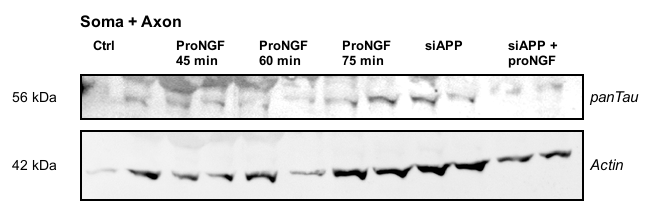
\includegraphics[width=0.8\linewidth,height=\textheight,keepaspectratio]{figures/feb1-show-1.png}

}

\caption{February 2026, 1st WB --- panTau (680 nm) and Actin (800 nm)
across soma and axon compartments.}

\end{figure}%

\subsection{Quantification}\label{quantification-1}

\begin{figure}[H]

{\centering \includegraphics[width=0.8\linewidth,height=\textheight,keepaspectratio]{figures/feb1-ratios-1.pdf}

}

\caption{February 2026, 1st WB --- panTau / Actin ratio in axon (left)
and soma (right) compartments.}

\end{figure}%

\begin{figure}[H]

{\centering \includegraphics[width=0.8\linewidth,height=\textheight,keepaspectratio]{figures/feb1-comparison-1.pdf}

}

\caption{February 2026, 1st WB --- Axon vs soma comparison for panTau
and Actin raw signals.}

\end{figure}%

\begin{center}\rule{0.5\linewidth}{0.5pt}\end{center}

\section{February 2026 --- 2nd Western Blot (Soma
Only)}\label{february-2026-2nd-western-blot-soma-only}

\textbf{Conditions:} Soma compartment only \textbf{Channel 680 nm:}
pTau65 (band 1) + pTau56 (band 2) \textbar{} \textbf{Channel 800 nm:}
pTau56 (band 1) + Actin (band 2)

\subsection{Blot Image}\label{blot-image-1}

\begin{figure}[H]

{\centering 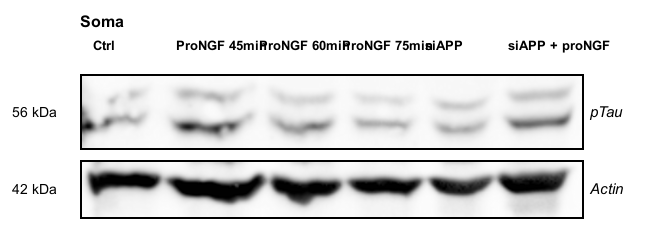
\includegraphics[width=0.8\linewidth,height=\textheight,keepaspectratio]{figures/feb2-show-1.png}

}

\caption{February 2026, 2nd WB --- pTau (680 nm) and Actin (800 nm),
soma compartment only.}

\end{figure}%

\subsection{Quantification}\label{quantification-2}

\begin{figure}[H]

{\centering \includegraphics[width=0.8\linewidth,height=\textheight,keepaspectratio]{figures/feb2-ratios-1.pdf}

}

\caption{February 2026, 2nd WB --- pTau56 / Actin (left) and total Tau /
Actin (right) in soma compartment.}

\end{figure}%

\begin{center}\rule{0.5\linewidth}{0.5pt}\end{center}

\section{Cross-Experiment Comparison --- Soma (February
2026)}\label{cross-experiment-comparison-soma-february-2026}

Comparing 1st WB (panTau/Actin) vs 2nd WB (Total Tau/Actin and
pTau56/Actin).

\begin{figure}[H]

{\centering \includegraphics[width=0.8\linewidth,height=\textheight,keepaspectratio]{figures/cross-ratio-1.pdf}

}

\caption{February 2026 --- Cross-experiment Tau / Actin comparison in
soma. 1st WB (panTau/Actin) vs 2nd WB (Total Tau/Actin and
pTau56/Actin).}

\end{figure}%

\begin{center}\rule{0.5\linewidth}{0.5pt}\end{center}

\section{Immunofluorescence --- p75 / Tau /
Tuj1}\label{immunofluorescence-p75-tau-tuj1}

\subsection{Control --- p75 / Tau / Tuj1 (Long
Axons)}\label{control-p75-tau-tuj1-long-axons}

\begin{figure}[H]

{\centering \includegraphics[width=1\linewidth,height=\textheight,keepaspectratio]{figures/if-ctrl-1.pdf}

}

\caption{Control condition --- immunofluorescence for p75 (AF568), Tau
(AF488), and Tuj1 (dodecane). Composite and individual channels shown.}

\end{figure}%

\subsection{BDNF + proNGF --- p75 / Tau /
Tuj1}\label{bdnf-prongf-p75-tau-tuj1}

\begin{figure}[H]

{\centering \includegraphics[width=1\linewidth,height=\textheight,keepaspectratio]{figures/if-bdnf-prongs-1.pdf}

}

\caption{BDNF + proNGF condition --- immunofluorescence for p75 (AF568),
Tau (AF488), and Tuj1 (dodecane).}

\end{figure}%

\subsection{BDNF --- p75 / Tau / Tuj1}\label{bdnf-p75-tau-tuj1}

\begin{figure}[H]

{\centering \includegraphics[width=1\linewidth,height=\textheight,keepaspectratio]{figures/if-bdnf-1.pdf}

}

\caption{BDNF condition --- immunofluorescence for p75 (AF568), Tau
(AF488), and Tuj1 (dodecane).}

\end{figure}%

\bookmarksetup{startatroot}

\chapter{Materials and Methods}\label{materials-and-methods}

\section{Experimental Design}\label{experimental-design}

\subsection{Neuronal cultures}\label{neuronal-cultures}

Wild-type pregnant rats were euthanized by exposure to CO2 and soaked in
70\% ethanol for 5 min for sterilization. Embryonic day 16 (E16) rat
fetuses were removed under sterile conditions and kept in
phosphate-buffered saline (PBS) on ice. Basal forebrains were dissected
and dissociated in serum-free medium (SFM) composed of a 1:1 mixture of
Eagle's MEM and Ham's F-12 supplemented with insulin (2.5μg/ml), glucose
(6 mg/ml), transferrin (100 μg/ml), putrescine (60 μm), progesterone (20
nm), selenium (30 nm), penicillin (0.5 U/ml), and streptomycin (0.5
μg/ml). The cells were then plated in microfluidic chambers (50)
attached to glass coverslips in tissue culture dishes that were
precoated overnight with poly-d-lysine (0.2 mg/ml). Two hundred
microliters of medium was added to the soma compartment, and 100 μl of
medium was maintained in the axon compartments to maintain a medium
volume difference that facilitated the growth of the axons of the
neurons through the microgrooves toward the axon compartment. The cells
were maintained with the volume difference between the soma and axon
compartments in SFM supplemented with 1\% B-27 for 5 days at 37°C to
obtain compartmentalized BFCN cultures that could be treated separately
at the axons or somas. For biochemical experiments, BFCNs were plated on
the top compartment of filter inserts with a pore size of 1 μm, allowing
neurites to grow through the filter to the bottom compartment, providing
an axon-enriched compartment for axon- or soma-specific stimulation
(51).

\subsection{Filter chamber cultures}\label{filter-chamber-cultures}

For axonal-specific treamtent experiments, BFCNs were plated on the top
compartment of Transwell filter inserts with a 1-μm pore size. Axons
grew through the pores to the bottom compartment over 5 days in vitro
(DIV). Compartmental separation of the filter system was validated in
prior study from our lab using 10-kDa dextran bead diffusion assays,
which established that diffusion from the axon to the soma compartment
is not detected until 2 hours, providing a 2-hour window for
axon-specific treatments (Dasgupta et al., 2024). This validation was
not repeated as part of the present thesis experiments.

\subsection{Immunocytochemistry}\label{immunocytochemistry}

Basal forebrain microfluidic cultures were fixed with 4\%
paraformaldehyde for 20 min, washed with PBS, and permeabilized with
0.5\% Triton X-100 in PBS for 10 min. Cells were blocked for 1 hour with
5\% normal goat serum and 1\% bovine serum albumin (BSA) in PBS. Cells
were then incubated overnight at 4°C with primary antibodies against
p75NTR (goat, 1:TODO) and Tau (rabbit, 1:TODO; TODO: clone/catalog)
diluted in 1\% BSA/PBS. The following day, cells were washed with PBS
and incubated for 1 hour at room temperature with a primary antibody
against β-tubulin III (Tuj1; mouse, 1:TODO; TODO: catalog). After
washing with PBS, cells were incubated for 1 hour at room temperature
with species-appropriate donkey secondary antibodies: donkey anti-goat
Alexa Fluor 488, donkey anti-rabbit Alexa Fluor 555, and donkey
anti-mouse Alexa Fluor 594 (all 1:TODO; Invitrogen). Coverslips were
mounted on slides with DAPI Fluoromount-G to label nuclei. Images were
acquired on a Zeiss LSM TODO confocal microscope at TODO×, and analyzed
using ImageJ software.

\subsection{Western blot analysis}\label{western-blot-analysis}

Five-DIV filter cultures were treated with proNGF, and axon and soma
lysates were obtained in 30 and 60 μl, respectively, of lysis buffer
composed of 10\% glycerol, 10\% Triton X-100, 10\% NP-40, 5\% 10×
protease inhibitors, and 5\% 10× phosphatase inhibitors. After protein
quantification, equal amounts of protein were run on a 12\%
polyacrylamide gel and transferred to nitrocellulose membrane. Equal
protein loading was assessed by Ponceau staining, which was washed out
with TBS (tris-buffered saline) with 0.05\% Tween 20 (TBST) and was
confirmed by re-probing the membranes with anti-actin. The membranes
were blocked with 5\% nonfat milk prepared in TBST for 1 hour. Membranes
were then incubated with primary antibodies diluted in blocking
solution. β-Actin (mouse, 1:TODO; catalog no. TODO) was incubated for 1
hour at room temperature. All other primary antibodies were incubated
overnight at 4°C and included: pan-Tau (mouse, 1:TODO; catalog no.
TODO), pan-Tau (rabbit, 1:TODO; catalog no. TODO), phospho-Tau (TODO
epitope; 1:TODO; catalog no. TODO), phospho-Tau (TODO epitope; 1:TODO;
catalog no. TODO), and phospho-Tau (TODO epitope; 1:TODO; catalog no.
TODO). After washing 3× 10 min with TBST, the blots were incubated with
appropriate secondary antibodies for 1 hour at room temperature. The
membrane was washed 3× 10 min with TBST and then scanned with the
Odyssey infrared imaging system (LI-COR Bioscience). All blots shown are
representative of at least three independent experiments.

\section{Statistical Analysis}\label{statistical-analysis}

\bookmarksetup{startatroot}

\chapter{Discussion}\label{discussion}

Discussion text.

\bookmarksetup{startatroot}

\chapter{Conclusion}\label{conclusion}

Conclusion text.

\bookmarksetup{startatroot}

\chapter*{References}\label{references}
\addcontentsline{toc}{chapter}{References}

\markboth{References}{References}

\phantomsection\label{refs}
\begin{CSLReferences}{1}{0}
\bibitem[\citeproctext]{ref-cagnettaRapidCueSpecificRemodeling2018}
Cagnetta, Roberta, Christian K. Frese, Toshiaki Shigeoka, Jeroen
Krijgsveld, and Christine E. Holt. 2018. {``Rapid {Cue-Specific
Remodeling} of the {Nascent Axonal Proteome}.''} \emph{Neuron} 99 (1):
29--46.e4. \url{https://doi.org/10.1016/j.neuron.2018.06.004}.

\bibitem[\citeproctext]{ref-Counts2011}
Counts, Scott E., and Elliott J. Mufson. 2011. {``The Role of Nerve
Growth Factor Signaling in Basal Forebrain Cholinergic Neuron
Degeneration in {Alzheimer}'s Disease.''} \emph{Current Alzheimer
Research} 8 (5): 514--25.

\bibitem[\citeproctext]{ref-dasguptaProNGFElicitsRetrograde2024}
Dasgupta, Srestha, Mansi A. Pandya, Juan P. Zanin, Tong Liu, Qian Sun,
Hong Li, and Wilma J. Friedman. 2024. {``{ProNGF} Elicits Retrograde
Axonal Degeneration of Basal Forebrain Neurons Through {p75NTR} and
Induction of Amyloid Precursor Protein.''} \emph{Science Signaling} 17
(855): eadn2616. \url{https://doi.org/10.1126/scisignal.adn2616}.

\bibitem[\citeproctext]{ref-Dechant2002}
Dechant, Geneviève, and Yves-Alain Barde. 2002. {``Neurotrophin
Signaling.''} \emph{Annual Review of Neuroscience} 25: 677--714.

\bibitem[\citeproctext]{ref-Ibanez1992}
Ibáñez, Carlos F. 1992. {``P75 Neurotrophin Receptor: A Multifunctional
Protein.''} \emph{Trends in Neurosciences} 15 (6): 217--23.

\bibitem[\citeproctext]{ref-Kaplan2013}
Kaplan, David R., and Frederick D. Miller. n.d. {``Neurotrophin Signal
Transduction in the Nervous System.''} \emph{Current Opinion in
Neurobiology} 23.

\bibitem[\citeproctext]{ref-Lei2016}
Lei, Peng et al. 2016. {``Tau Phosphorylation and Aggregation in
{Alzheimer}'s Disease.''} \emph{Acta Neuropathologica} 131: 1--14.

\bibitem[\citeproctext]{ref-Morfini2009}
Morfini, Gerardo A. et al. 2009. {``Axonal Transport Defects in
Neurodegenerative Diseases.''} \emph{Journal of Neuroscience} 29 (41):
12776--86.

\bibitem[\citeproctext]{ref-Teng2005}
Teng, Helen K. et al. 2005. {``{ProNGF} Induces Neuronal Apoptosis via
Activation of the {p75NTR}--Sortilin Complex.''} \emph{Journal of
Neuroscience} 25 (22): 5455--63.

\bibitem[\citeproctext]{ref-tengProBDNFInducesNeuronal2005}
Teng, Henry K., Kenneth K. Teng, Ramee Lee, Saundrene Wright, Seema
Tevar, Ramiro D. Almeida, Pouneh Kermani, et al. 2005. {``{ProBDNF}
Induces Neuronal Apoptosis via Activation of a Receptor Complex of
{p75NTR} and Sortilin.''} \emph{The Journal of Neuroscience: The
Official Journal of the Society for Neuroscience} 25 (22): 5455--63.
\url{https://doi.org/10.1523/JNEUROSCI.5123-04.2005}.

\bibitem[\citeproctext]{ref-Yaar1997}
Yaar, Menachem et al. 1997. {``Expression of P75 Neurotrophin Receptor
in the Adult Human Brain.''} \emph{Journal of Neuroscience} 17 (13):
4813--24.

\end{CSLReferences}




\end{document}
